\documentclass[12pt]{article}

\usepackage{times}
\usepackage{textcomp}
\usepackage{listings}
\usepackage{fullpage}
\usepackage{color}
\usepackage{hyperref} 
\usepackage{pst-tree} 
\usepackage{verbatim} 
\usepackage{graphicx}
\usepackage{amsmath,amsfonts,amssymb,amsthm}
\graphicspath{ {./}} 

\def\part#1{\item[\bf #1)]}
\renewcommand{\thesubsection}{Question \arabic{subsection}}

\author{Clement Tsang}

\begin{document}

\begin{center}
\Large\textbf{CS 241, Lecture 9 - Maximal Munch and Context Free Grammars}
\end{center}
\begin{center}
\textbf{Tues, Feb 05, 2019}
\end{center}

\section{Maximal Munch and Simplified Maximal Munch}
\begin{itemize}
    \item The general idea is to consume the largest possible token that makes sense, then produce the token and then proceed.
    \item Maximal munch differs from simplified maximal munch:
        \begin{itemize}
            \item Maximal munch consumes chars until there is no valid transition.  If there are still characters, backtrack to the last valid accepting state and resume.
            \item Simplified maximal munch consumes chars until there is no longer a valid transition.  If the state is accepting, produce the token and proceed.  Otherwise go to error state.
        \end{itemize}
    \item Observe the following DFA for $w$ = ``ababca'':\\
        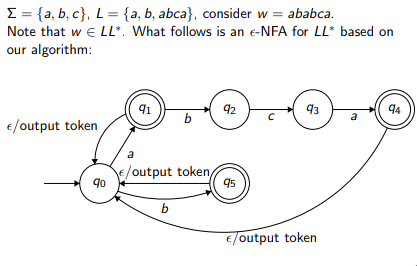
\includegraphics[scale=0.8]{maxmunch1.png} 
    \item With SMM, when we hit the second ``a'', we stop and output an error, which is not the correct answer.
    \item With MM, the second ``a'' is reached, and the last accepting state was ``a''.  We backtrack back to ``a'' and resume munch (go back to $q_0$, resume by consuming ``b''.  We would have to keep track of the last accepting state.
    \item Note SMM is usually good enough and thus we typically use this without issue - that is, we make our language work with SMM rather than the other way around.
    \item Examples of the MM and SMM algorithms: \\
        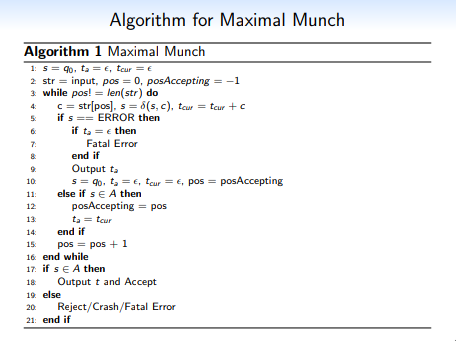
\includegraphics[scale=0.8]{mmalg.png} \\
        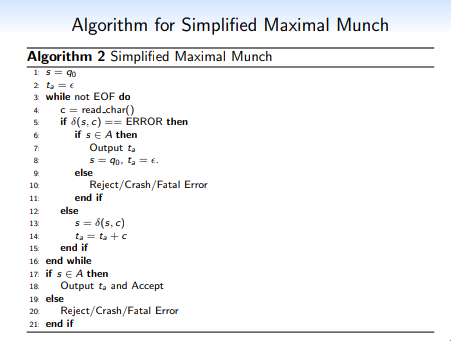
\includegraphics[scale=0.8]{smmalg.png}
    \item This concludes the process of scanning. 
\end{itemize}

\section{Syntactic Analysis - Context-Free Grammars}
\begin{itemize}
    \item Things we have to consider: syntax (is the order of tokens correct, are parentheses balanced?) and semantics (does what is written make sense?).
    \item A \textbf{grammar} is the language of languages - they help us describe what we are and are not allowed to say.
    \item \textbf{Context-free grammars} is a 4-tuple $(N, \Sigma, P, S)$ where:
        \begin{itemize}
            \item $N$ is a finite non-empty set of non-terminal symbols (symbols you cannot stop on)
            \item $\Sigma$ is an alphabet, or in other words a set of non-empty terminal symbols, and $N \hat Z = \emptyset$.
            \item $P$ is a finite set of productions, each of the form $A \rightarrow \beta$ where $A \in N$ and $\beta \in (N \cup \Sigma)*$.
            \item $S \in N$ is a starting symbol.
        \end{itemize}
    \item We set $V = N \cup \Sigma$ to denote the vocabulary - the set of \emph{all} symbols in our language.
    \item For example, in rustcc, we defined various CFGs, such as Fn containing BlockItems which contained Statements or Declarations which contained...
    \item \textbf{Conventions}:
        \begin{itemize}
            \item Lower case letters from the start of the alphabet are elements of $\Sigma$
            \item Lower case letters from the end of the alphabet are elements of $\Sigma^*$ (words)
            \item Upper case letters from the start of the alphabet are elements of $N$
            \item $S$ is always our start symbol
            \item Greek letters like $\alpha, \beta, \gamma$ are elements of $V^* = (N \cup \Sigma)^*$.
        \end{itemize}
    \item For example, consider $\Sigma = \{(, )\}$, and let $L = \{w : w \text{ is a balance string of parentheses}\}$.  Thus, $S \rightarrow \epsilon, S \rightarrow (S), S \rightarrow SS \Rightarrow S \rightarrow \epsilon | (S) | SS$ 
    \item A \textbf{derivation} over a CFG$(N, \Sigma, P, S)$ is such that:
        \begin{itemize}
            \item $\alpha$ derives $\beta$ and we write $\alpha \Rightarrow \beta$ iff $\beta$ can be obtained from $\alpha$ using a rule from $P$.
            \item $\alpha A \beta \Rightarrow \alpha \gamma \beta$ iff there is a rule $A \rightarrow \gamma$ in $P$.
            \item $\alpha \Rightarrow^* \beta$ iff a derivation exists, that is, there exists $\delta_i \in V^*$ for $0 \leq i \leq k$ such that $\alpha = \delta_0 \Rightarrow \delta_1 \Rightarrow \dots \Rightarrow \delta_k = \beta$.  Note $k$ can be 0.
        \end{itemize} 
    \item Another example: find a derivation of (()()).  Recall our above CFG:
        \begin{align*}
            S & \Rightarrow (S) \Rightarrow (SS) \Rightarrow ((S)S) \\
              & \Rightarrow ((S)(S)) \Rightarrow ((\epsilon)(S)) \\
              & \Rightarrow (()()) \\
            S & \Rightarrow^* (()()) \quad\text{, short form for the above implications}
        \end{align*}
    \item Why is it ``context-free''?  It's because our grammar does not care for the context - that is, it does not care for \emph{where} your symbols are.
    \item This is the opposite of \textbf{context-bounded grammars}, which is where the context of the other symbols around other symbols \emph{will} affect our productions (note we don't \emph{really} need to know about this)
    \item We define the \textbf{language} of a CFG$(N, \Sigma, P, S)$ to be $L(G) = \{w \in \Sigma^* : S \Rightarrow^* w\}$.
    \item A language is \textbf{context-free} iff there exists a CFG $G$ such that $L = L(G)$.
    \item Informally, we can show regular languages are context-free: \\
        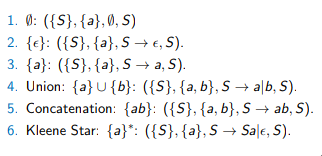
\includegraphics[scale=0.8]{cg.png}
\end{itemize}

\end{document}

